% vim: expandtab tabstop=2 softtabstop=2 shiftwidth=2
\documentclass[aspectratio=169]{beamer}
\usepackage[frenchb,noconfigs]{babel}
\usepackage{ifluatex,ifxetex}
\ifnum 0\ifxetex 1\fi\ifluatex 1\fi=0 % if pdftex
  \usepackage[utf8]{inputenc}
  \usepackage[T1]{fontenc}
\fi
\usepackage{relsize,xcolor}

\usepackage{beamerx}

\newcommand\typographix{\raisebox{-1.4ex}[0pt][0pt]{
\includegraphics[height=4ex]{typographix.pdf}}}

\title[Documents and slides]
      {{\rm\LaTeX} january sessions}
      [LaTeX, by TypographiX]
\author{Clément Durand, binet \typographix{}}

\setbeamerfont{footnote}{size=\tiny}
\begin{document}
\maketitle

\begin{frame}{Why would you use \LaTeX~?}
  You would use \LaTeX{} if~:\pause{}
  \begin{itemize}[<+->]
    \item You expect a \emph{high typographical quality} of your documents without too much effort~;
    \item You want to \emph{focus on the content} of your productions~;
    \item You intend to write \emph{long or scientific} texts, or want a simple way to use \emph{biography, table of content, index or references}.
  \end{itemize}
\end{frame}

\begin{frame}{How about the format~?}\centering%
  \emph{My school wants me to produce documents with a specific layout.}\bigskip

  \emph{I want beautiful documents and slides.}
\end{frame}

\begin{frame}{What TypographiX has to offer.}\centering%
  \setlength\unitlength{0.01\textwidth}
  \begin{picture}(100,45)
    \put(2,40){\makebox(0,0)[tl]{%
        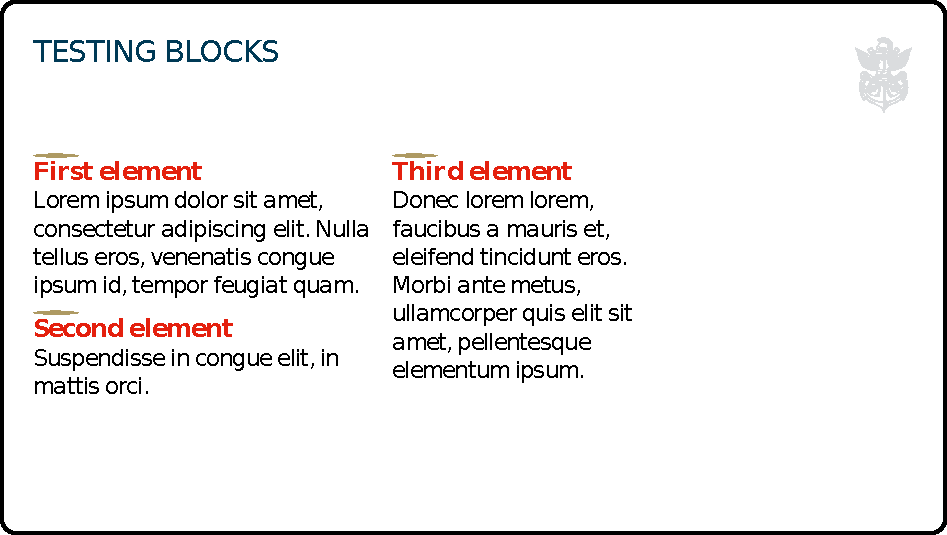
\includegraphics[width=0.35\textwidth]{sli2.pdf}%
    }}%
    \put(0,5){\makebox(0,0)[bl]{%
        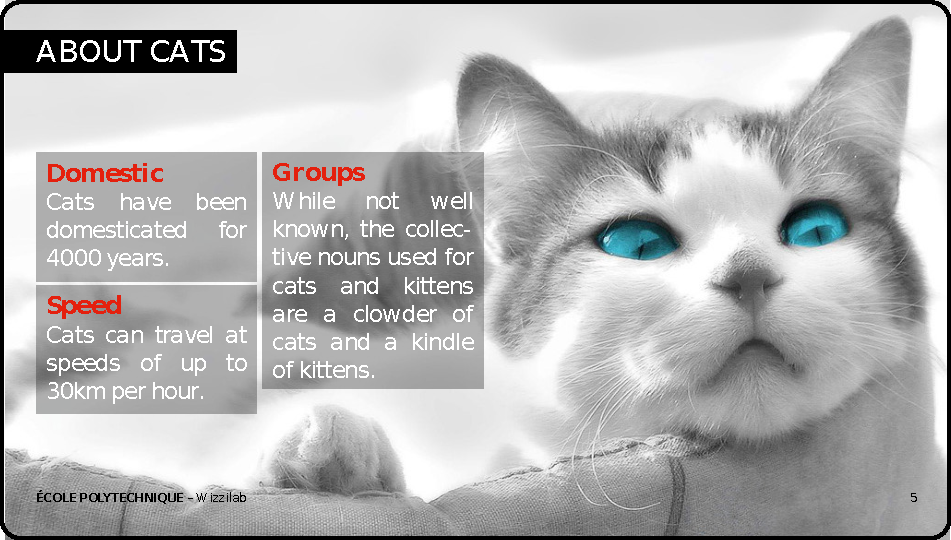
\includegraphics[width=0.35\textwidth]{sli1.pdf}%
    }}%
    \put(98,22.5){\makebox(0,0)[cr]{%
        
\includegraphics[width=0.26\textwidth]{doc1.pdf}%
    }}%
    \put(55,22.5){\makebox(0,0)[c]{%
        \begin{minipage}{0.3\textwidth}\centering%
          Automated layout of your documents and slides. You can now focus on content~!
        \end{minipage}
    }}%
  \end{picture}
\end{frame}

\begin{frame}{Why and when wouldn't you use \LaTeX~?}
  You wouldn't use \LaTeX{} if~:\pause{}
  \begin{itemize}[<+->]
    \item You don't want to \emph{spend a little time} to learn to use it~;
    \item Your document is \emph{already ready} and pretty~;
    \item You want to \emph{control and create a specific design}.
  \end{itemize}
\end{frame}

\end{document}
